\documentclass[11pt]{beamer}\usepackage[]{graphicx}\usepackage[]{color}
%% maxwidth is the original width if it is less than linewidth
%% otherwise use linewidth (to make sure the graphics do not exceed the margin)
\makeatletter
\def\maxwidth{ %
  \ifdim\Gin@nat@width>\linewidth
    \linewidth
  \else
    \Gin@nat@width
  \fi
}
\makeatother

\definecolor{fgcolor}{rgb}{0.345, 0.345, 0.345}
\newcommand{\hlnum}[1]{\textcolor[rgb]{0.686,0.059,0.569}{#1}}%
\newcommand{\hlstr}[1]{\textcolor[rgb]{0.192,0.494,0.8}{#1}}%
\newcommand{\hlcom}[1]{\textcolor[rgb]{0.678,0.584,0.686}{\textit{#1}}}%
\newcommand{\hlopt}[1]{\textcolor[rgb]{0,0,0}{#1}}%
\newcommand{\hlstd}[1]{\textcolor[rgb]{0.345,0.345,0.345}{#1}}%
\newcommand{\hlkwa}[1]{\textcolor[rgb]{0.161,0.373,0.58}{\textbf{#1}}}%
\newcommand{\hlkwb}[1]{\textcolor[rgb]{0.69,0.353,0.396}{#1}}%
\newcommand{\hlkwc}[1]{\textcolor[rgb]{0.333,0.667,0.333}{#1}}%
\newcommand{\hlkwd}[1]{\textcolor[rgb]{0.737,0.353,0.396}{\textbf{#1}}}%

\usepackage{framed}
\makeatletter
\newenvironment{kframe}{%
 \def\at@end@of@kframe{}%
 \ifinner\ifhmode%
  \def\at@end@of@kframe{\end{minipage}}%
  \begin{minipage}{\columnwidth}%
 \fi\fi%
 \def\FrameCommand##1{\hskip\@totalleftmargin \hskip-\fboxsep
 \colorbox{shadecolor}{##1}\hskip-\fboxsep
     % There is no \\@totalrightmargin, so:
     \hskip-\linewidth \hskip-\@totalleftmargin \hskip\columnwidth}%
 \MakeFramed {\advance\hsize-\width
   \@totalleftmargin\z@ \linewidth\hsize
   \@setminipage}}%
 {\par\unskip\endMakeFramed%
 \at@end@of@kframe}
\makeatother

\definecolor{shadecolor}{rgb}{.97, .97, .97}
\definecolor{messagecolor}{rgb}{0, 0, 0}
\definecolor{warningcolor}{rgb}{1, 0, 1}
\definecolor{errorcolor}{rgb}{1, 0, 0}
\newenvironment{knitrout}{}{} % an empty environment to be redefined in TeX

\usepackage{alltt}
\usetheme{Warsaw}
\usepackage[utf8]{inputenc}
\usepackage{amsmath}
\usepackage{amsfonts}
\usepackage{amssymb}
\usepackage{array}
\author{John Muschelli}
\setbeamertemplate{navigation symbols}{}%remove navigation symbols

\title{File Formats of Neuroomaging}
%\setbeamercovered{transparent} 
%\setbeamertemplate{navigation symbols}{} 
%\logo{} 
\institute{Johns Hopkins Bloomberg School of Public Health} 
%\date{} 
%\subject{} 
\setlength{\topsep}{0pt}
\setlength{\parskip}{0pt}
\setlength{\partopsep}{1pt}
\IfFileExists{upquote.sty}{\usepackage{upquote}}{}
\begin{document}

\begin{frame}
\titlepage
\end{frame}

%\begin{frame}
%\tableofcontents
%\end{frame}



\begin{frame}[fragile]{Image formats: DICOM}
DICOM (Digital Imaging and Communications in Medicine) format

\begin{itemize}
\item Standardized way of representing images
\item Usually how data is given either from scanner or hospital PACS (picture archiving and communication system) system 
\item 2 integral pieces: Image data (in pixels) and header (meta-data (data about data))
\begin{itemize}
	\item Think of a JPEG and a text file
\end{itemize}
%\item Extensions are usually \verb|.dcm|, but may have no extension whatsoever
\end{itemize}

\end{frame}


\begin{frame}[fragile]{DICOM pixel data}

The pixel data in a DICOM file is a matrix (fixed number of rows and columns). 

One DICOM file represents one "slice" of the brain.

The \verb|oro.dicom| package is good for reading in this data.

\begin{knitrout}
\definecolor{shadecolor}{rgb}{0.969, 0.969, 0.969}\color{fgcolor}\begin{kframe}
\begin{alltt}
\hlkwd{library}\hlstd{(oro.dicom)}
\hlstd{slice} \hlkwb{=} \hlkwd{readDICOM}\hlstd{(}\hlstr{'Example_DICOM.dcm'}\hlstd{)}
\hlkwd{class}\hlstd{(slice)}
\end{alltt}
\begin{verbatim}
[1] "list"
\end{verbatim}
\end{kframe}
\end{knitrout}

\end{frame}

\begin{frame}[fragile]{readDICOM output}

The output is a list with 2 elements: the DICOM header (\verb|hdr|) and image (\verb|img|) information, both of which are lists.

Each element of \verb|hdr| has a \verb|data.frame|, and the elements of \verb|img| are matrices:
\begin{knitrout}
\definecolor{shadecolor}{rgb}{0.969, 0.969, 0.969}\color{fgcolor}\begin{kframe}
\begin{alltt}
\hlkwd{names}\hlstd{(slice)}
\end{alltt}
\begin{verbatim}
[1] "hdr" "img"
\end{verbatim}
\begin{alltt}
\hlkwd{class}\hlstd{(slice}\hlopt{$}\hlstd{hdr)}
\end{alltt}
\begin{verbatim}
[1] "list"
\end{verbatim}
\begin{alltt}
\hlkwd{class}\hlstd{(slice}\hlopt{$}\hlstd{hdr[[}\hlnum{1}\hlstd{]])}
\end{alltt}
\begin{verbatim}
[1] "data.frame"
\end{verbatim}
\begin{alltt}
\hlkwd{class}\hlstd{(slice}\hlopt{$}\hlstd{img)}
\end{alltt}
\begin{verbatim}
[1] "list"
\end{verbatim}
\begin{alltt}
\hlkwd{class}\hlstd{(slice}\hlopt{$}\hlstd{img[[}\hlnum{1}\hlstd{]])}
\end{alltt}
\begin{verbatim}
[1] "matrix"
\end{verbatim}
\end{kframe}
\end{knitrout}

\end{frame}

\begin{frame}[fragile]{Display DICOM Image}

We can display the data using the \verb|image| command.  

(We transpose the data using \verb|t()| so the image faces ``up'' instead of ``right''.)

\begin{knitrout}
\definecolor{shadecolor}{rgb}{0.969, 0.969, 0.969}\color{fgcolor}\begin{kframe}
\begin{alltt}
\hlkwd{image}\hlstd{(}\hlkwd{t}\hlstd{(slice}\hlopt{$}\hlstd{img[[}\hlnum{1}\hlstd{]]),} \hlkwc{col}\hlstd{=}\hlkwd{gray}\hlstd{(}\hlnum{0}\hlopt{:}\hlnum{64}\hlopt{/}\hlnum{64}\hlstd{))}
\end{alltt}
\end{kframe}
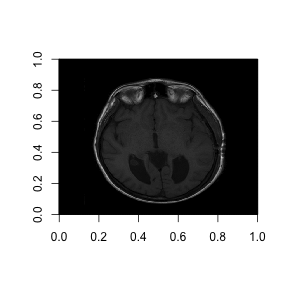
\includegraphics[width=.8\linewidth]{figure/display_dicom-1} 

\end{knitrout}

\end{frame}

\begin{frame}[fragile]{DICOM Header Information}

What about the header?

There are many fields, for example pixelSpacing, which is the dimensions (x and y) of a pixel in millimeters (mm):

\begin{knitrout}
\definecolor{shadecolor}{rgb}{0.969, 0.969, 0.969}\color{fgcolor}\begin{kframe}
\begin{alltt}
\hlstd{hdr} \hlkwb{=} \hlstd{slice}\hlopt{$}\hlstd{hdr[[}\hlnum{1}\hlstd{]]}
\hlstd{hdr[ hdr}\hlopt{$}\hlstd{name} \hlopt{==} \hlstr{'PixelSpacing'}\hlstd{,} \hlstr{"value"}\hlstd{]}
\end{alltt}
\begin{verbatim}
[1] "0.46875 0.46875"
\end{verbatim}
\end{kframe}
\end{knitrout}

\end{frame}


\begin{frame}[fragile]{Multiple DICOM files}

We have discussed only one slice of the brain.  What about multiple slices?  If you pass a directory into \verb|readDICOM|, it will read in all DICOM files in that directory.

\begin{knitrout}
\definecolor{shadecolor}{rgb}{0.969, 0.969, 0.969}\color{fgcolor}\begin{kframe}
\begin{alltt}
\hlstd{all_slices} \hlkwb{=} \hlkwd{readDICOM}\hlstd{(}\hlstr{'T1/'}\hlstd{)}
\end{alltt}
\end{kframe}
\end{knitrout}


\end{frame}



\begin{frame}[fragile]{NIfTI}

Now that we have multiple files read in, we can convert it to a 3-dimensional (3D) array, where you can think of the array as stacking each slice (which is a matrix) on top of each other.  If each DICOM is a piece of paper, the 3D array is a stack of paper.\\

The way we store this 3D array is in the NIfTI (Neuroimaging Informatics Technology Initiative) format.  \\

\begin{table}[h]
\begin{tabular}{m{0.15\textwidth}|m{0.42\textwidth}|m{0.42\textwidth}}
& DICOM & NIfTI \\ \hline
File extension: & .dcm & .nii or .nii.gz (compressed) \\
Each file is a: & slice of the brain & 3D image of brain \\
Header information: & Many fields, protected health information, hospital-related meta-data & Image meta-data, no patient information \\
Different Images & Different Folders & Different Files (can be same directory)
\end{tabular}
\end{table}
\end{frame}

\begin{frame}[fragile]{NIfTI}

We can convert this list of header information and image information to a \verb|nifti| object (an R object) with the \verb|dicom2nifti| command:
\begin{knitrout}
\definecolor{shadecolor}{rgb}{0.969, 0.969, 0.969}\color{fgcolor}\begin{kframe}
\begin{alltt}
\hlstd{nii} \hlkwb{=} \hlkwd{dicom2nifti}\hlstd{(all_slices)}
\end{alltt}


{\ttfamily\noindent\bfseries\color{errorcolor}{Error in nim@pixdim[2:4] <- attr(img, "{}pixdim"{}): could not find function "{}checkAtAssignment"{}}}\begin{alltt}
\hlkwd{dim}\hlstd{(nii);} \hlkwd{class}\hlstd{(nii)}
\end{alltt}


{\ttfamily\noindent\bfseries\color{errorcolor}{Error in eval(expr, envir, enclos): object 'nii' not found}}

{\ttfamily\noindent\bfseries\color{errorcolor}{Error in eval(expr, envir, enclos): object 'nii' not found}}\end{kframe}
\end{knitrout}
We can see that this \verb|nii| object is indeed a \verb|nifti| object and has 3 dimensions. 

\end{frame}

\begin{frame}[fragile]{NIfTI}

Now that we have multiple files read in, we can convert it to a 3-dimensional (3D) array, where you can think of the array as stacking each slice (which is a matrix) on top of each other.  If each DICOM is a piece of paper, the 3D array is a stack of paper.\\

The way we store this 3D array is in the NIfTI (Neuroimaging Informatics Technology Initiative) format.  \\

\begin{table}[h]
\begin{tabular}{m{0.15\textwidth}|m{0.42\textwidth}|m{0.42\textwidth}}
& DICOM & NIfTI \\ \hline
File extension: & .dcm & .nii or .nii.gz (compressed) \\
Each file is a: & slice of the brain & 3D image of brain \\
Header information: & Many fields, protected health information, hospital-related meta-data & Image meta-data, no patient information 
\end{tabular}
\end{table}
\end{frame}







\begin{frame}[fragile]{Other formats}

For Philips scanners, files from the scanner are PAR/REC and not DICOM.  \verb|dcm2nii| can convert to NIfTI. \\

NIfTI format was based on ANALYZE fromat where the header and image were in separate \verb|.hdr| and \verb|.img| files.  This is an older fromat and we will not use this way of storing data because 1) NIfTI can have one file with both header and image information, and 2) Can be stored as compressed .nii.gz files.\\

NRRD (Nearly Raw Raster Data) is another format similar to NIfTI.  Much of the neuroimaging software can read in both NRRD and NIfTI files, but NIfTI is much more common.

\end{frame}


\end{document}
